\chapter{شروع کار با یونیتی}
حالا شما مراحل نصب را پشت سر گذاشته‌اید و اگر پا به پای این کتاب پیش رفته باشید، در صفحهٔ ورود اوبونتو قرار دارید.
\begin{center}
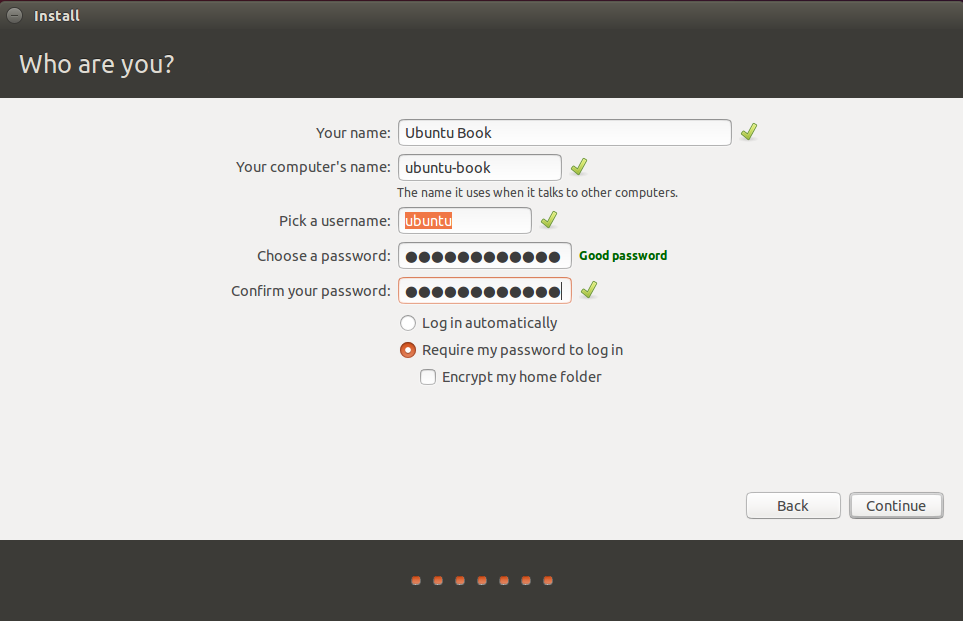
\includegraphics[scale=0.4]{pics/11.jpg}
\end{center}

بعد از واردکردن گذرواژه، وارد صفحهٔ زیر می‌شوید. این همان یونیتی است؛ محیطی که به طور پیش‌فرض در اوبونتو با آن کار خواهید کرد.
\begin{center}
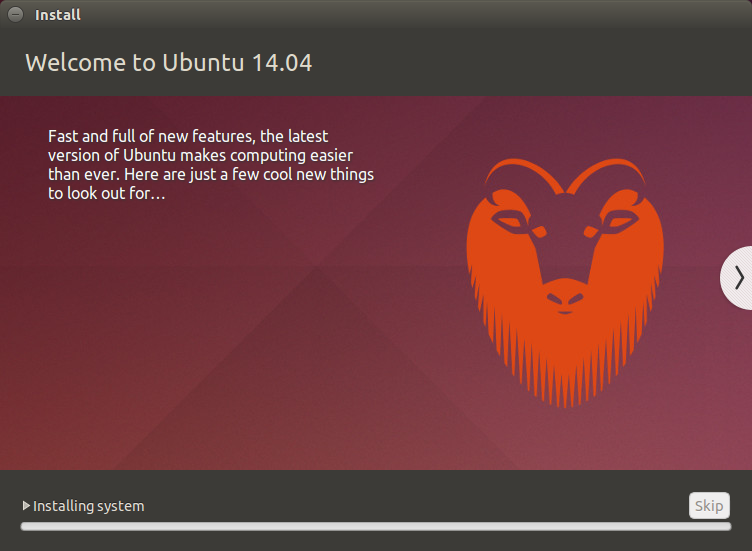
\includegraphics[scale=0.4]{pics/12.jpg}
\end{center}

\section{یونیتی چیست؟}
یونیتی محیطی است که سادگی، زیبایی، قدرت و یکپارچگی را هم برای کاربران و هم برای توسعه دهندگان نرم‌افزار فراهم می‌کند.
هیچ جای نگرانی نیست؛ یونیتی تماماً ویژگی‌های محیط‌های قبلی را که با آن‌ها احتمالاً در ویندوز یا سیستم عامل اپل کار کرده‌اید، دارد. ویژگی‌هایی مانند کشیدن و رهاکردن، کلیک‌کردن روی آیکون‌ها، قابلیت کپی‌کردن و بسیاری دیگر.
در ادامه بیش‌تر با یونیتی آشنا خواهید شد.
\subsection{تاریخچهٔ یونیتی}
شاید برای‌تان جالب باشد که یونیتی از کجا آمده است، چه گروهی آن را توسعه می‌دهند و از ابتدا روی اوبونتو بوده است.\\
یونیتی محیط کاری است که در حال حاضر تنها روی توزیع اوبونتو در دسترس است و توسط تیم اوبونتو در حال توسعه است. یونیتی یکی از جوان ترین محیط‌های کاری است. در‌واقع، یونیتی از توزیع ۱۱/۰۴ روی اوبونتو قرار گرفت و عمری کمتر از ۳ سال دارد؛ اما توانسته در همین مدت کوتاه، محیطی بسیار ساده، زیبا و کارآمد را به کاربران خود ارائه دهد. یونیتی با هدفِ رفتن اوبونتو بر روی دستگاه‌های دیگر (تبلت‌ها و گوشی‌ها و تلویزیون‌های هوشمند) و ظاهری یکپارچه برای تمامی دستگاه‌ها طراحی شده است و در هر نسخه، به ویژگی‌ها و پایداری آن افزوده می‌شود. اوبونتو ۱۳/۱۰ از نسخه ۷ یونیتی استفاده می‌کند.
\section{واسط کاربری یونیتی}
ظاهر یونیتی شامل بخش‌های زیر است:
\begin{itemize}
\item میزکار
\item اجراگر (\lr{Launcher})
\item پنل
\item داشبورد
\item هود
\end{itemize}

\subsection{میزکار}
محیط اصلی شماست. در این محیط، شما می‌توانید برنامه‌ها و پنجره‌های مختلف را باز یا بسته کنید.
\subsection[اجراگر (Launcher)]{اجراگر (\lr{Launcher})}
اجراگر همان سکویی است که در سمت چپ به صورت عمودی قابل مشاهده است. در لانچر، تمام برنامه‌های باز شما نمایش داده می‌شود. همچنین شما می‌توانید برنامه‌هایی را که بیش‌تر به آن‌ها نیاز دارید، در آن‌جا نگه دارید تا با سرعت بیش‌تری به آن‌ها دسترسی داشته باشید.
\subsubsection{راهنمای اجراگر}
برای اضافه و حذف کردن آیکن یک برنامه به اجراگر، کافی است روی لوگوی اوبونتو کلیک کنید و نام یا ویژگی برنامهٔ مورد نظر خود را تایپ کنید و بعد، آیکن آن برنامه را با موس گرفته و به روی اجراگر بکشید و رهایش کنید. برای حذف‌کردن نیز تنها کافیست روی آن آیکن، کلیک راست موس را بزنید و روی \lr{Unlock from Launcher} کلیک کنید؛ یا این‌که آیکن را گرفته و آن را بر روی آیکن سطل زباله برده و رها کنید تا آیکن برنامه از اجراگر حذف شود.
\subsection{هود}
فرایند گشتن در منوهای تودرتو و پیچیده و به خاطر سپردن موقعیت زیرمنوها، همیشه کاری بیهوده و زمانبر بوده است. یونیتی با هود به شما امکان جست‌و‌جوی سریع و بی‌دردسر را در منوها می‌دهد. با زدن کلید \lr{Alt} در پنجرهٔ برنامهٔ در حال اجرا، \lr{Hud} را فعال کرده و در منوهای آن پنجره جست‌وجو کنید.
\begin{center}
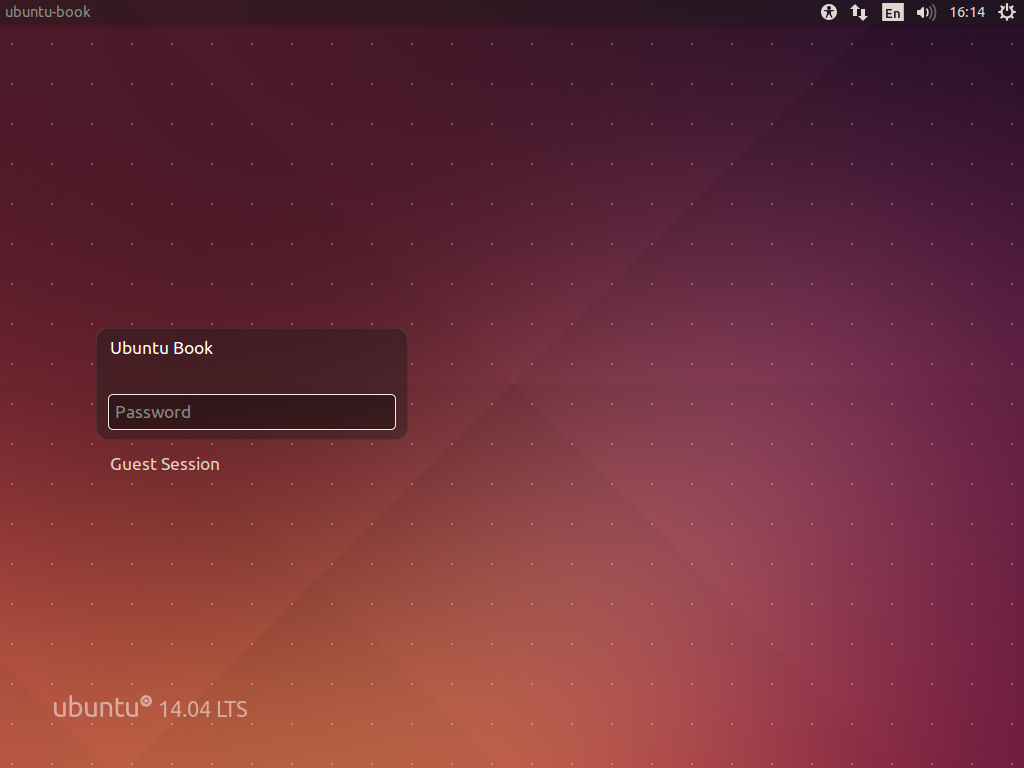
\includegraphics[scale=0.43]{pics/13.jpg}
\end{center}

\subsection{پنل}
پنل همان نواری است که در بالاترین قسمت از محیط خود آن را می‌بینید. در پنل، اطلاعاتی مانند منوی تنظیمات، ساعت و تاریخ ، صدا، شبکه و منوی من که برای اطلاع از آخرین وضیعت پیام‌های پست الکترونیکی و شبکه‌های اجتماعی و چت با دوستان‌تان است. اما شاید مهم‌ترین چیزی که در پنل به آن نیاز دارید، منوی پنجره‌ای است که در آن مشغول به کار هستید.

\subsubsection{ویژگی‌های پنل}
پنل از دو بخش تشکیل شده است: بخش سمت راست که در آن منوی تنظیمات، منوی کاربر، ساعت و تاریخ، تنظیمات صدا، تنظیمات شبکه، منوی من، نمایش باتری (در صورت استفاده از لپ‌تاپ) و تغییر زبان قرار گرفته و در سمت چپ، منوی برنامه وجود دارد که ابتدا نام پنجره فعال در آن نمایان است؛ اما با بردن موس بر روی سمت چپ پنل، این منو نمایان می‌شود. این قابلیت یونیتی باعث می‌شود که وقتی به منو احتیاجی ندارید، از دید پنهان باشد.
\begin{description}
\item[منوی من] \hfill \\
در منوی من که به شکل یک پاکت نامه در بالا نمایان است، به موارد زیر دسترسی خواهید داشت:
\begin{itemize}
\item نوع وضعیت در برنامه‌های گفت‌وگو (چت)
\item دسترسی و مدیریت حساب‌های شبکه‌های اجتماعی
\item دسترسی و مدیریت پست الکترونیکی
\item دسترسی به برنامه‌های تحت وب نصب‌شدهٔ مرتبط
\end{itemize}
این پاکت نامه، در صورتی که پیغامی خوانده نشده داشته باشید، به رنگ آبی در می آید. همچنین شما می توانید با کلیک وسط موس روی این پاکت نامه، به نشانه اطلاع‌تان از پیغام، رنگ‌اش را به رنگ اولیه تغییر دهید.
\begin{center}
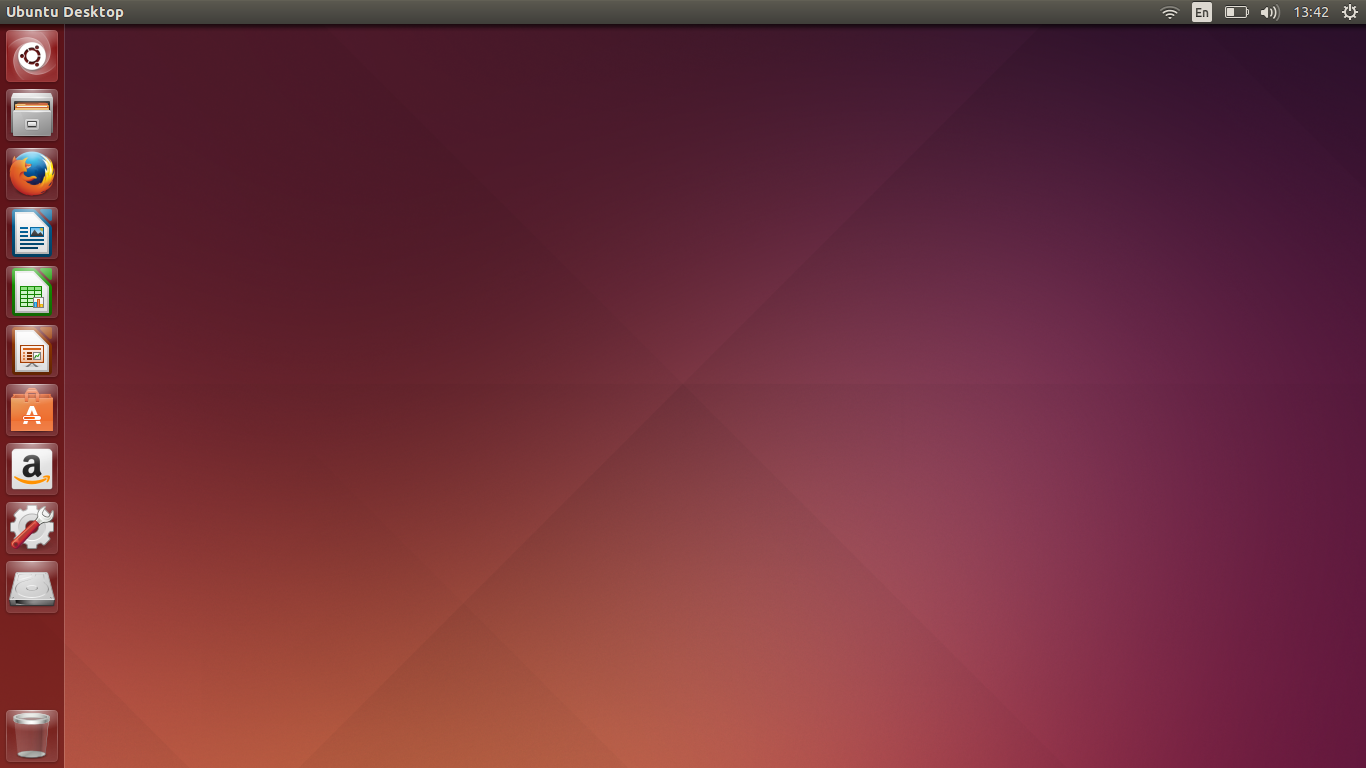
\includegraphics[scale=0.43]{pics/14.jpg}
\end{center}

\item[نشانگر شبکه] \hfill \\
شما در این منو می‌توانید شبکهٔ بی‌سیم خود را انتخاب کنید و با وارد کردن گذرواژه، از این شبکه بی‌سیم استفاده کنید. همچنین، این منو دسترسی سریع شما را به تنظیمات شبکه و \lr{VPN} فراهم می‌کند.
\begin{center}
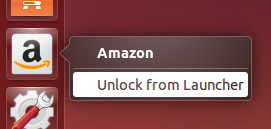
\includegraphics[scale=0.43]{pics/15.jpg}
\end{center}

\item[نشانگر صدا] \hfill \\
در این نشانگر، قادر خوهید بود صدا را کم یا زیاد کنید. همچنین امکان پخش و یا تغییر آهنگ در حال پخش نیز وجود دارد.
\begin{center}
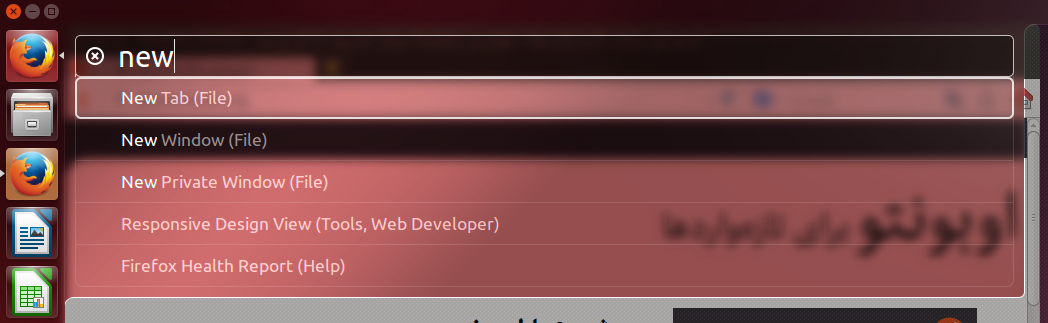
\includegraphics[scale=0.43]{pics/16.jpg}
\end{center}

\item[نشانگر ساعت] \hfill \\
در این نشانگر شما به تنظیمات ساعت، تاریخ و تقویم ماهانه دسترسی خواهید داشت.
\begin{center}
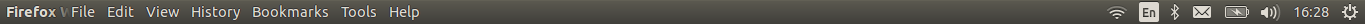
\includegraphics[scale=0.43]{pics/17.jpg}
\end{center}

\item[نشانگر تنظیمات] \hfill \\
شما در این نشانگر، به تنظیمات صفحه نمایش، تنظیمات سیستم، بروزرسانی، چاپگر و خاموش کردن یا شروع مجدد سیستم و سوییچ‌کردن از یک حساب کاربری به حساب کاربری دیگر دسترسی دارید.
\begin{center}
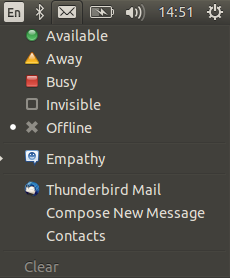
\includegraphics[scale=0.43]{pics/18.jpg}
\end{center}

\end{description}

\subsection{داشبورد}
داشبورد واسطی است که سریع‌ترین و راحت‌ترین دسترسی به فایل‌ها و برنامه‌ها را برای کاربران فراهم می‌کند. شما به کمک داشبورد می‌توانید نام برنامه یا کلمهٔ کلیدی آن را جست‌وجو کنید. همچنین می‌توانید برای جست‌وجوی خود، محدودیت‌هایی را اعمال کنید تا فقط در آن دسته به دنبال نتیجه باشید. همچنین با بازشدن داشبورد، به فایل‌ها و برنامه‌هایی که به تازگی استفاده کرده‌اید، دسترسی خواهید داشت.
\begin{center}
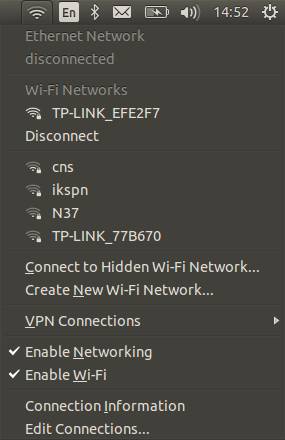
\includegraphics[scale=0.43]{pics/19.jpg}
\end{center}

\subsubsection{نحوهٔ دسترسی به داشبورد}
شما برای دسترسی به داشبورد، می‌توانید از ۲ راه استفاده کنید؛ راه اول این‌که می‌توانید با استفاده از موس، روی بالاترین آیکون در لانچر (آیکون اوبونتو) کلیک کنید و داشبورد نمایان خواهد شد. همچنین می‌توانید در کیبورد روی دکمهٔ ویژه (که دکمهٔ ویندوز هم نامیده می‌شود) کلیک کنید تا داشبورد نمایان شود.

\subsubsection{ظاهر داشبورد}
داشبورد از بخش‌های زیر تشکیل شده است:
\begin{itemize}
\item جست‌وجو
\item نمایشگر
\item فیلتر
\item \textbf{لنزها}\\
دش به طور پیش فرض ۶ لنز دارد که هر لنز، برای دسترسی سریع‌تر شما به هدف‌تان طراحی شده است. این ۶ لنز عبارت‌اند از: لنز خانه که امکان دسترسی به آخرین فایل‌ها و برنامه‌ها را دارد، لنز برنامه که تنها برای نرم‌افزارهاست، لنز فایل که تنها بین فایل‌های شما جست‌وجو می کند، لنز موسیقی که فایل‌ها موسیقی شما را پیدا می‌کند، لنز عکس بین عکس‌های شما می گردد و همین‌طور لنز فیلم که بین فیلم‌هایی که روی دستگاه شما قرار دارد و فیلم‌هایی که با آن موضوع در فضای اینترنت قرار دارد، جست‌وجو را انجام می‌دهد.
\end{itemize}

\subsubsection{پیش‌نمایش}
امکان مشاهدهٔ پیش‌نمایشی از محتواهای مختلف، با کلیک راست روی آن در داشبورد وجود دارد. مثلا با کلیک راست روی آیکن \lr{Chromium} در داشبورد، توضیحاتی از آن به همراه اسکرین‌شات و امتیاز کسب‌شده از کاربران نشان داده می‌شود. پیش‌نمایش از برنامه‌ها، تصاویر، ویدیو، موزیک و تعدادی دیگر از قالب ها پشتیبانی می‌کند.

\subsection{برنامه‌های تحت وب}
با کمک برنامه‌های تحت وب یا \lr{WebApps}، می‌توان وب‌سایت‌هایی مانند \lr{Gmail}، \lr{Grooveshark}، \lr{Last.fm}، \lr{Facebook} و بسیاری دیگر را با محیط \lr{Unity} یکپارچه کرد. برای مثال با نصب \lr{WebApp}های مناسب، می‌توانید \lr{Grooveshark} را با منو صدا کنترل و پیام ها جدید \lr{Google+}‎ را با سیستم اعلان اوبونتو دریافت نمایید. دو \lr{WebApp} فروشگاه موسیقی \lr{Ubuntu One} و \lr{Amazon}، به صورت پیش‌فرض فعال هستند. \lr{WebApp} های بیش‌تر، از مرکز نرم‌افزاری قابل نصب هستند؛ اما راه راحت‌تر آن است که با مرورگر \lr{Firefox}، سایت مورد نظر خود را، مانند \lr{Gmail}، باز کنید که بعد از آن، پیشنهاد نصب (در صورت موجود بودن برنامه برای آن وب‌سایت) به شما داده می‌شود.
